\chapter{Real-Time Ethernet} \label{ch:realTimeEthernet}

Ethernet is a networking standard used in local area networks (LAN) that can a support a real-time system using packet switching, high bandwidth and low interference. We will look at the history of Ethernet and what challenges lay back then, a single segment Ethernet setup with CSMA/CD technology, then multi segment Ethernet with the spanning-tree protocol (STP) and a implementation of it.

\section{The history of Ethernet and single segment}

Ethernet was developed at Xerox PARC in 1973 and commercially introduced in 1980 as the so-called "DIX" (Digital, Intel, Xerox) standard with a bandwidth of 10Mbit/s, using coaxial cables and described as a technology for local-area networks". Ethernet became dominant over the likes of Token Ring and Token Bus in the end of the 1980's, because Ethernet was more adaptive than these proprietary protocols and quickly switched to the twisted-pair wiring (UTP, unshielded twisted pair), reducing cost, complexity and boosting transmission rates.

\noindent The Ethernet standard was intended for a typical office environment with workstations, but did also support PC-based controllers, PLC's and other devices, because it was an open-standard and easily accessible. Figure X illustrates a Plant-Control-Device environment, with higher response times at the plant level, more data transfers but less frequency.

\begin{figure}[h!]\label{}
	\centering
	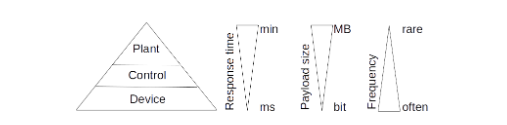
\includegraphics[scale=0.5]{realTimeEthernet/PlantControlDevice.png}
	\caption{The plant, control and device segments of a domain. Plant span entire facilities, control span plant floors and device span parts of plant floor.}
	\label{fig:plantcontroldevice}
\end{figure}

\noindent The first mid-80's Ethernet technologies (10BASE2, 10BASE5, and early 10BASE-T) constituted a so-called single segment network and relied on hubs, repeaters and the CSMA/CD (Carrier Sense Multiple Access with Collision Detection) protocol for sharing bandwidth on a shared medium. It was relatively low cost and flexible, but nondeterministic medium access made it hard to guarantee deadlines and use in a real-time system with no packet prioritization. Also speed was a function of the number of nodes on a network link. When sending, CSMA/CD implements carrier-sense by listening on the network for traffic. If it occurs, it does not transmit data. If no traffic for a certain period, it transmits data. Multiple Access allows more nodes to share the medium, but means collisions are more likely and that all packets are passed to all nodes. To mitigate this, the protocol brings Collision Detection, where a node listens for collisions on the medium, if they occur it sends a jam signal, back-offs for a random time period (exponential back-off algorithm) and tries again.

\noindent The truncated exponential back-off algorithm (EBA) retransmits after a random back-off time given by:

\[ T_{back-off}: r \times T_{slot} \]

\noindent with these properties:

\begin{itemize}
	\item $T_{slot}$ = $T_{dataout}$ + $T_{jam-back}$. The time it takes for the data to be sent to the point of collision and for the jam signal to get back. It is the max theoretical round-trip time.
	\item r $\sim$ \textit{u}[0, ..., 2\^{c} - 1], where \textit{u} is a uniform distribution.
	\item c is a local node counter, c $\in$ [1;$c_max$], and is reset after successful transmission. $c_max$ = 10 in the IEEE 802.3 CSMA/CD standard. Truncation means that after a certain number of increases, exponentiation stops and is reset.
\end{itemize}

\noindent For 10Mbit/s Ethernet, $T_{slot}$ = 51.2$\mu$s and decreases when transmission rates $\longrightarrow$ $\propto$. Figure \ref{fig:csmacd} shows how a collision on the wire, how the two re-transmissions collide and the random back-off timer in effect.

\begin{figure}[h!]\label{}
	\centering
	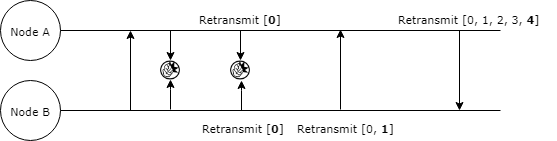
\includegraphics[scale=0.5]{realTimeEthernet/CSMACD.png}
	\caption{CSMA/CD in effect with random re-transmissions upon collisions.}
	\label{fig:csmacd}
\end{figure}

\noindent A conceivable drawback of the back-off algorithm is that it can introduce medium monopolization by one node in a network, $Node_{a}$, depriving another node, $Node_{b}$ of time to send. As the back-off algorithm is random, if $Node_{a}$ is more successful than $Node_{b}$ at sending packets, $Node_{b}$'s collision counter might increase beyond that of $Node_{a}$, resulting in exponential wait times for $Node_{b}$. In the next chapter we look at how to solve collisions using network segmentation.



\section{Multi-segment Ethernet and STP}
\subsection{Multi-segment}

To solve issues with collisions it is neccessary to split the network into different domains each with their own collision domains. This was made possible with the introduction of switches which segmented the network on the Link layer (OSI Level 2) in 1990 by Kalpana, which was later acquired by Cisco. The segmentation resulted in traffic no longer being broadcast across multiple nodes, and at the extreme each node is connected directly to a network switch forming a micro segment. In 1998 full 8 wire twisted pair wires were introduced which allowed for Pysical layer (OSI Level 1) segmentation as the cables were now full duplex. In the years since the price of CAT 5 cables and switches has dropped, and eventually the older technologies were phased out in most networks, removing all potential for collisions. To ensureAs a consequence of the collision free networks it became possible to exceed 10 Mbps and modern networking cards support 100 Mbps at a minimum and 1 Gbps is becoming more common. To insure thees network speeds there was made spanning-tree protocol (STP) which is building for making forwarding topology free-loop and for reducing broadcast radiation. 

\subsection{Spanning-tree protocol}
The idea behind the STP protocol is to have only one way from one node to another one. As in the Figure \ref{fig:STP} A is before the algorithm B is after the algorithm. The STP finds the fastest and loop-free path between two nodes.

Kruskal's algorithm:

\begin{enumerate}
	\item Sort the edges by weight, increasing, and add them to a list.
	\item Add the edge with the lowest weight from the list and remove it from the list hereafter.	
	\item Add the next edge with the lowest weight if adding the edge does not create a circle and remove it from the list hereafter.
	\item Repeat 4 step until a minimum spanning tree has been formed.
\end{enumerate}

The algorithm was made during the course using networkx library in python the Figure\ref{fig:STP} shows graphical example for our implementation of Kruskal's algorithm.

\begin{figure}[H]\label{}
	\centering
	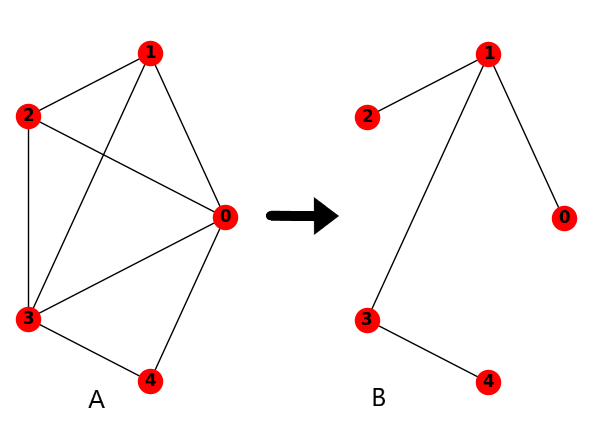
\includegraphics[scale=0.5]{realTimeEthernet/Image/STP.png}
	\caption{Spanning-tree protocol exercise}
	\label{fig:STP}
\end{figure}


\section{Multi-segment real-time Ethernet}

%Maybe put this together with multiSegmentStp?

To solve issues with collisions it is neccessary to split the network into different domains each with their own collision domains. This was made possible with the introduction of switches which segmented the network on the Link layer (OSI Level 2) in 1990 by Kalpana, which was later acquired by Cisco. The segmentation resulted in traffic no longer being broadcast across multiple nodes, and at the extreme each node is connected directly to a network switch forming a micro segment. In <Year> full 8 wire twisted pair wires were introduced which allowed for Pysical layer (OSI Level 1) segmentation as the cables were now full duplex. In the years since the price of CAT 5 cables and switches has dropped, and eventually the older technologies were phased out in most networks, removing all potential for collisions. As a consequence of the collision free networks it became possible to exceed 10 Mbps and modern networking cards support 100 Mbps at a minimum and 1 Gbps is becoming more common.

\subsection{Store and forward vs. Cut through}

Switches have two modes of operation, 'store and forward' mode or 'cut through' mode. Both modes have their own advantages and disadvantages with neither being objectively better. 

* Store and forward: In this mode the switch stores each package and verifies that it has been received correctly. If the package has been corrupted then the switch will request a retransmission from the previous node. This mode minimizes the transmission of corrupted packages, reducing the overall congestion in the network and improving the performance in a high noise environment. The downsides are that this mode is resource intensive from the switch which increases latency and throughput, especially when there is much traffic on the network.
* Cut through: In this mode the switch starts sending the package as soon as it starts receiving it, reducing latency and saving resources for data transmissions. This reduction in latency (down to 10 ms between two nodes) makes Cut through more suitable to real time systems. The downsides of cut through switching is that corrupted packages will also be transmitted along with other traffic allowing corrupt data to get further through the network before being caught and retransmitted. 

Many switches have the ability to switch between store and forward and cut through modes depending on the context.

A major challenge for switches is the need to manage routing of messages to the correct recievers, preferably without being manually configured to do so. The switch will manage a list of MAC addresses reachable from each port by monitoring the sender addresses of incoming packages. When in doubt the switch will simply broadcast the message to all active ports aside from the sender. Due to these broadcasts there is a risk of the network flooding itself in cases where 

